\section{Phương pháp đề xuất}\label{sec:ours}

\subsection{Động cơ}
Khi khai báo có cạnh thiếu, cách an toàn nhất là đưa lag của \emph{cả $n$ nút} vào mọi phương trình để không đường truyền nào bị bỏ sót. Với $n=14$ và $T=40$, cách này đưa $28$ biến hồi quy lag vào $38$ dòng dữ liệu, phương sai hệ số tăng vọt và khoảng tin cậy rất rộng. \ours{} dựa trên hai ý: (i) chỉ mở khối lag cho các cặp biến có bằng chứng từ dữ liệu, với số cặp mở được định bởi số cạnh thiếu khai báo; (ii) chạy lại việc chọn cấu trúc trong từng lần bootstrap, để khoảng tin cậy gộp cả nhiễu dữ liệu lẫn bất định về cấu trúc.

\begin{figure}[H]
\centering
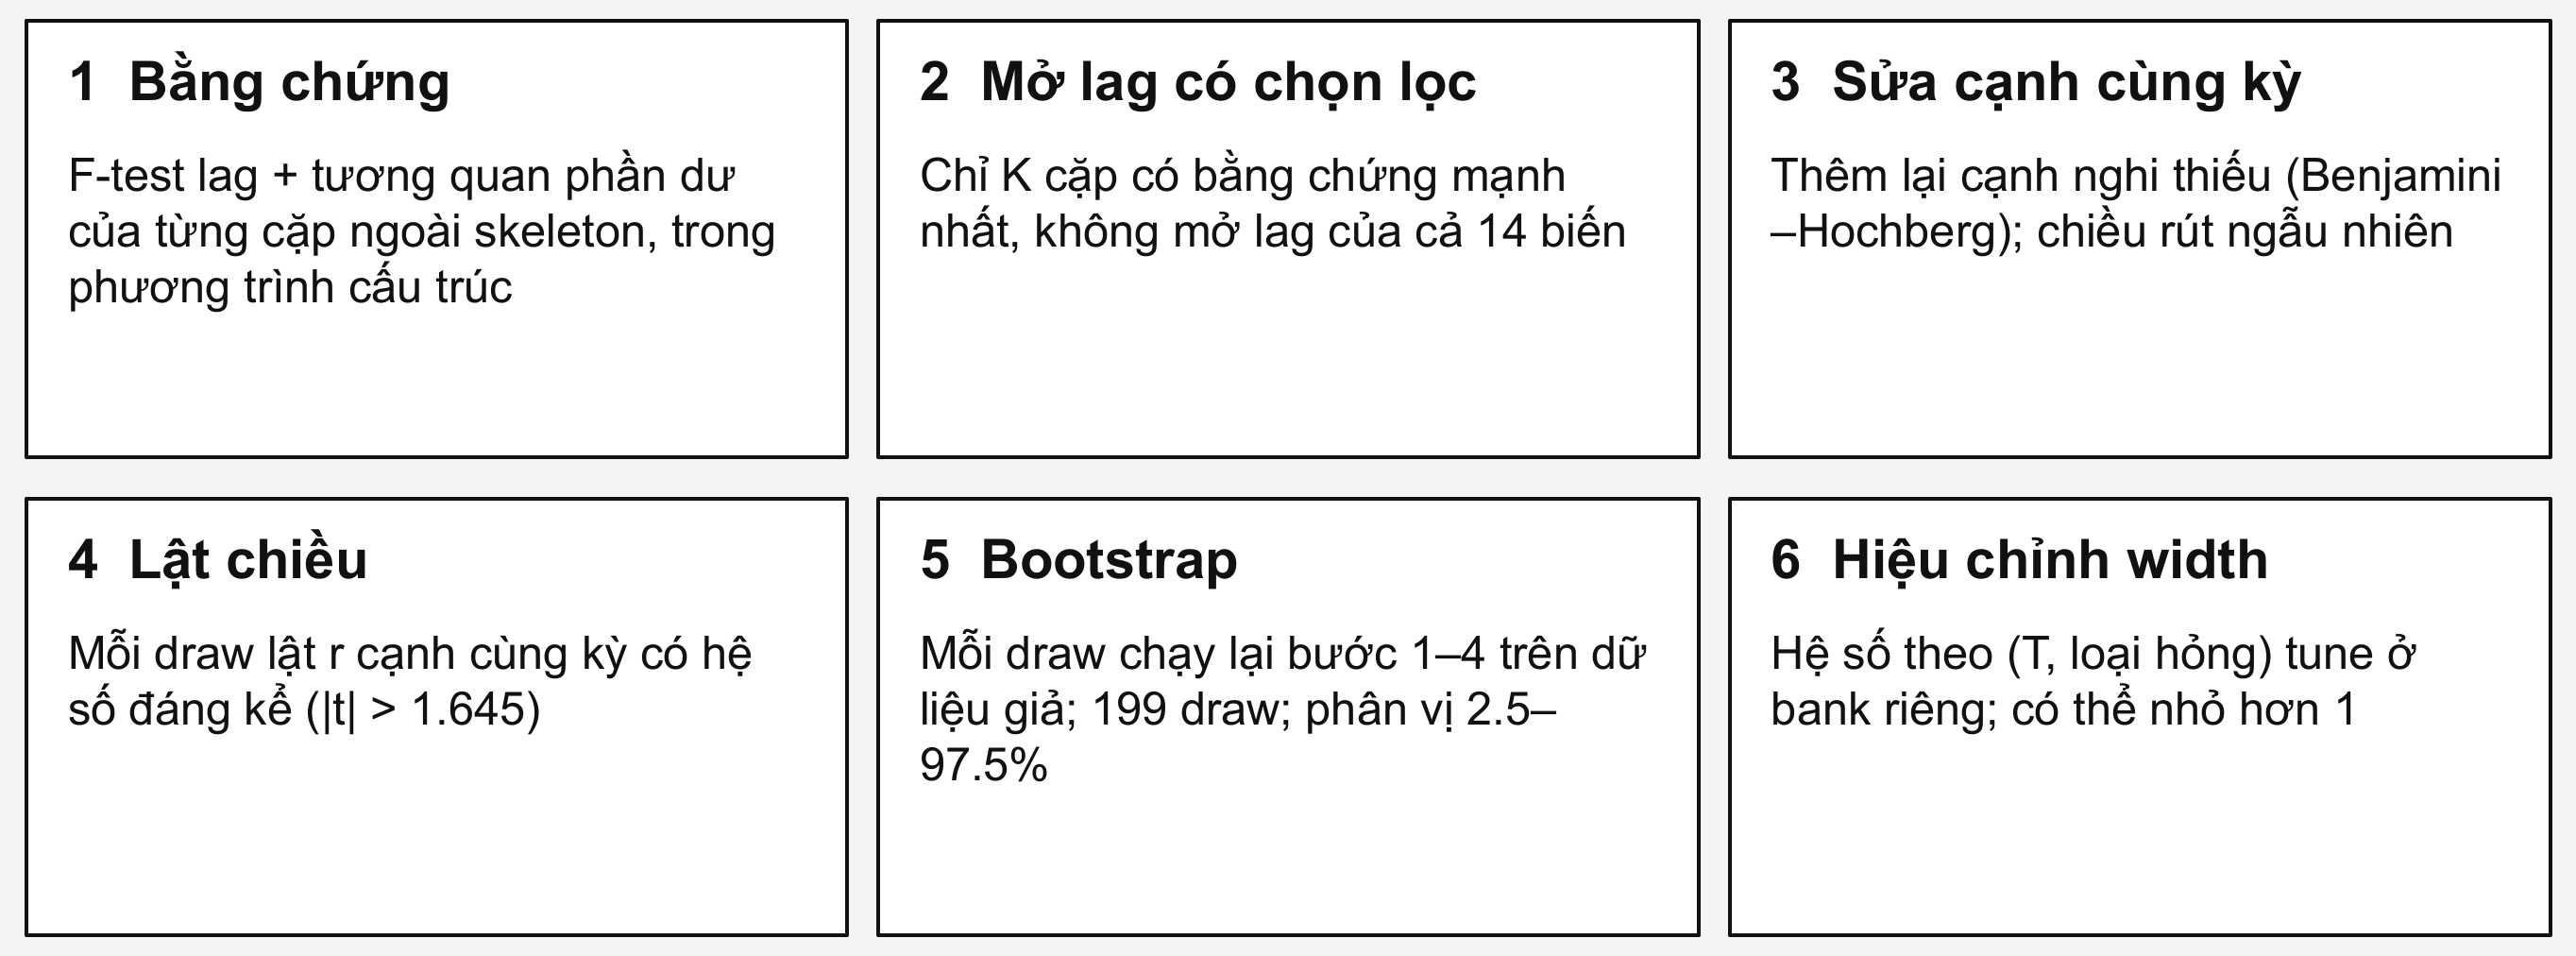
\includegraphics[width=\textwidth]{figures/buoc_phuong_phap_ours.png}
\caption{Sáu bước của \ours{}.}\label{fig:ours}
\end{figure}

Đầu vào gồm dữ liệu $X\in\mathbb R^{T\times n}$, skeleton $\mathcal S$ (với tập cạnh cùng kỳ có hướng $\mathcal O$) và khai báo $(k_{\text{miss}},k_{\text{extra}},k_{\text{rev}})$. Gọi $\mathcal N$ là tập các cặp \emph{không nối} trong $\mathcal S$. Đầu ra là $\hat C_{ji}(H)$ và $[\ell_{ji},u_{ji}]$ cho mọi cặp có thứ tự.

\subsection{Bước 1: chấm bằng chứng cho từng cặp không nối}
Với mỗi cặp $\{u,v\}\in\mathcal N$, chúng tôi chạy ba kiểm định \emph{trong phương trình cấu trúc của skeleton} (lag của chính nút, lag của các cặp nối, các cha cùng kỳ của skeleton):
\begin{enumerate}
  \item F-test thêm khối lag của $u$ vào phương trình của $v$;
  \item F-test thêm khối lag của $v$ vào phương trình của $u$;
  \item Fisher $z$ trên tương quan giữa phần dư cấu trúc của $u$ và của $v$ (dấu vết của một cạnh cùng kỳ bị thiếu).
\end{enumerate}
Ba $p$-value $p_1,p_2,p_3$ được gộp bằng phép hiệu chỉnh Šidák \citep{sidak1967rectangular}:
\begin{equation}
p_{uv}=1-\bigl(1-\min(p_1,p_2,p_3)\bigr)^3.
\end{equation}
Phân phối F được xấp xỉ bằng xấp xỉ chuẩn của Paulson. Kiểm định được đặt trong phương trình cấu trúc thay vì trong reduced-form VAR, vì ở reduced-form hiệu ứng truyền qua cạnh cùng kỳ làm các cặp không nối nhau trông như có quan hệ Granger, nên test không còn là test về sự kề nhau.

\subsection{Bước 2: mở khối lag có chọn lọc (targeted lag opening)}
Sắp xếp các cặp theo $p_{uv}$ tăng dần và mở khối lag (cả hai chiều) cho $K$ cặp đầu:
\begin{equation}
K=\min\Bigl(|\mathcal N|,\ \max\bigl(\lceil 3k_{\text{miss}}\rceil,\ \#\{p_{uv}<0.10\}\bigr)\Bigr).
\end{equation}
Số cạnh thiếu khai báo đặt \emph{sàn} cho lượng được mở ($3k_{\text{miss}}$); bằng chứng mạnh có thể mở nhiều hơn.

\subsection{Bước 3: bổ sung cạnh cùng kỳ (contemporaneous repair)}
Cạnh cùng kỳ bị thiếu để lại tương quan giữa các phần dư cấu trúc. Chúng tôi kiểm định các cặp không nối bằng thủ tục Benjamini--Hochberg \citep{benjamini1995controlling} ở mức $q=0.1$ rồi thêm lại tối đa $k_{\text{miss}}$ cạnh, mạnh nhất trước. Dữ liệu không xác định chiều của các cạnh này, nên mỗi lần chạy bootstrap rút chiều ngẫu nhiên; nếu chiều rút tạo chu trình thì lấy chiều còn lại.

\subsection{Bước 4: đảo chiều có chọn lọc (targeted reversal)}
Khi $k_{\text{rev}}>0$, mỗi lần chạy bootstrap lật $k_{\text{rev}}$ cạnh cùng kỳ, chọn trong các cạnh có hệ số cùng kỳ đáng kể ($|t|>1.645$ ở lần fit đầu) và không tạo chu trình.

\subsection{Bước 5: bootstrap có chọn lại cấu trúc}
Mỗi lần chạy bootstrap sinh dữ liệu giả $X^*$ từ phần dư (mục~\ref{sec:bootstrap}), rồi \emph{làm lại các bước 1--4 trên $X^*$} (chọn lại $K$ cặp, bổ sung cạnh, đảo chiều) và fit để được $\hat C^*(H)$. Với $B=199$ lần chạy, khoảng tin cậy là phân vị $2.5\%$--$97.5\%$ và điểm ước lượng là trung bình của các lần. Vì cấu trúc được chọn lại trong từng lần, khoảng tin cậy phản ánh nhiễu dữ liệu và bất định về cấu trúc, tức khoảng hiệu ứng trên các skeleton khả dĩ quanh skeleton đã cho.

\subsection{Bước 6: hiệu chỉnh độ rộng hai phía}
Khoảng từ bước 5 được co về trung điểm với hệ số $0.5$, rồi nhân với hệ số $c(T,\text{loại lỗi})$ chọn trên một tập dữ liệu hiệu chỉnh riêng, không dùng để chấm điểm, bằng lưới $1.0$--$10$ bước $0.1$. Hệ số hiệu dụng $0.5$--$5$ có thể nhỏ hơn 1, nên bước này nới được khoảng khi under-cover và thu hẹp được khi over-cover. Ví dụ khi thiếu cạnh, hệ số hiệu dụng là $1.3$ ở $T=80$ và $1.15$ ở $T=150$. Các hệ số được cố định trước và không chỉnh lại trên dữ liệu kiểm chứng; loại lỗi dùng để chọn hệ số là thành phần khai báo lớn nhất.

\begin{algorithm}[H]
\caption{\ours{}}
\begin{algorithmic}[1]
\Require $X$, skeleton $\mathcal S$, khai báo $(k_{\text{miss}},k_{\text{rev}})$, $B=199$
\State $\mathrm{Select}(X)\gets$ bước 1--3: tính $p_{uv}$, mở $K$ cặp, chọn ứng viên bổ sung cạnh
\State fit trên $X$ với skeleton, các cặp được mở và một lần rút cạnh bổ sung; thu $\hat B$ và phần dư $\hat u$
\For{$b=1,\dots,B$}
  \State $X^*\gets$ dựng chuỗi giả từ $\hat B$ và phần dư rút có hoàn lại
  \State $(\text{cặp mở}^*,\text{cạnh bổ sung}^*)\gets \mathrm{Select}(X^*)$ \Comment{chọn lại cấu trúc}
  \State rút chiều cho cạnh bổ sung; lật $k_{\text{rev}}$ cạnh (bước 4)
  \State fit trên $X^*$, tính $\hat C^{*(b)}(H)$ bằng \eqref{eq:irf}--\eqref{eq:cumulative}
\EndFor
\State $[\ell,u]\gets$ phân vị $2.5\%$, $97.5\%$ của $\{\hat C^{*(b)}\}$
\State co về trung điểm với hệ số $0.5$, rồi nhân $c(T,\text{loại lỗi})$ đã cố định
\State \Return $\hat C=\overline{\hat C^{*(b)}}$ và $[\ell,u]$
\end{algorithmic}
\end{algorithm}

\subsection{Trường hợp đặc biệt}
Khi không khai báo cạnh thiếu ($k_{\text{miss}}=0$), các bước 2--3 không chạy; phương pháp chỉ đảo chiều có chọn lọc rồi hiệu chỉnh độ rộng ở bước 6. Mỗi lần gọi mất khoảng $1.3$--$1.4$ giây ở $T=80$--$150$ với $n=14$ (bảng~\ref{tab:budget}).
